

\tikzset{every picture/.style={line width=0.75pt}} %set default line width to 0.75pt        

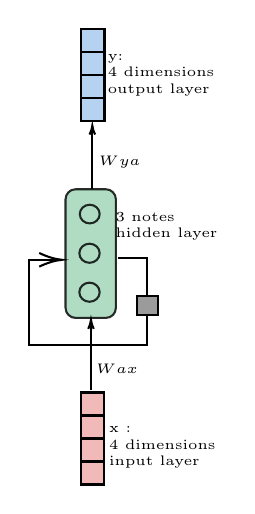
\begin{tikzpicture}[x=0.75pt,y=0.75pt,yscale=-1,xscale=1]
%uncomment if require: \path (0,300); %set diagram left start at 0, and has height of 300

%Rounded Rect [id:dp5767801512845814] 
\draw  [color={rgb, 255:red, 0; green, 0; blue, 0 }  ,draw opacity=0.82 ][fill={rgb, 255:red, 78; green, 178; blue, 121 }  ,fill opacity=0.45 ][line width=0.75]  (117.57,131.31) .. controls (117.57,128.63) and (119.74,126.46) .. (122.42,126.46) -- (136.98,126.46) .. controls (139.66,126.46) and (141.83,128.63) .. (141.83,131.31) -- (141.83,183.6) .. controls (141.83,186.28) and (139.66,188.46) .. (136.98,188.46) -- (122.42,188.46) .. controls (119.74,188.46) and (117.57,186.28) .. (117.57,183.6) -- cycle ;
%Shape: Ellipse [id:dp18804427153778946] 
\draw  [color={rgb, 255:red, 0; green, 0; blue, 0 }  ,draw opacity=0.82 ] (124.44,138.43) .. controls (124.44,135.95) and (126.58,133.93) .. (129.23,133.93) .. controls (131.88,133.93) and (134.02,135.95) .. (134.02,138.43) .. controls (134.02,140.91) and (131.88,142.92) .. (129.23,142.92) .. controls (126.58,142.92) and (124.44,140.91) .. (124.44,138.43) -- cycle ;
%Shape: Ellipse [id:dp672728185189052] 
\draw  [color={rgb, 255:red, 0; green, 0; blue, 0 }  ,draw opacity=0.82 ] (124.22,176.07) .. controls (124.22,173.53) and (126.41,171.47) .. (129.12,171.47) .. controls (131.83,171.47) and (134.02,173.53) .. (134.02,176.07) .. controls (134.02,178.61) and (131.83,180.67) .. (129.12,180.67) .. controls (126.41,180.67) and (124.22,178.61) .. (124.22,176.07) -- cycle ;
%Shape: Ellipse [id:dp22457931655016228] 
\draw  [color={rgb, 255:red, 0; green, 0; blue, 0 }  ,draw opacity=0.82 ] (124.22,157.3) .. controls (124.22,154.76) and (126.41,152.7) .. (129.12,152.7) .. controls (131.83,152.7) and (134.02,154.76) .. (134.02,157.3) .. controls (134.02,159.84) and (131.83,161.9) .. (129.12,161.9) .. controls (126.41,161.9) and (124.22,159.84) .. (124.22,157.3) -- cycle ;
%Shape: Rectangle [id:dp3603601739458042] 
\draw  [fill={rgb, 255:red, 234; green, 141; blue, 141 }  ,fill opacity=0.61 ] (124.9,224.38) -- (136.12,224.38) -- (136.12,235.47) -- (124.9,235.47) -- cycle ;
%Shape: Rectangle [id:dp3229189908551803] 
\draw  [fill={rgb, 255:red, 234; green, 141; blue, 141 }  ,fill opacity=0.61 ] (124.9,235.47) -- (136.12,235.47) -- (136.12,246.56) -- (124.9,246.56) -- cycle ;
%Shape: Rectangle [id:dp21435953126093987] 
\draw  [fill={rgb, 255:red, 234; green, 141; blue, 141 }  ,fill opacity=0.61 ] (124.9,246.56) -- (136.12,246.56) -- (136.12,257.64) -- (124.9,257.64) -- cycle ;
%Shape: Rectangle [id:dp23717670155716364] 
\draw  [fill={rgb, 255:red, 234; green, 141; blue, 141 }  ,fill opacity=0.61 ] (124.9,257.64) -- (136.12,257.64) -- (136.12,268.73) -- (124.9,268.73) -- cycle ;

%Shape: Rectangle [id:dp5297698591025225] 
\draw  [fill={rgb, 255:red, 148; green, 188; blue, 234 }  ,fill opacity=0.68 ] (125.11,49.12) -- (136.33,49.12) -- (136.33,60.21) -- (125.11,60.21) -- cycle ;
%Shape: Rectangle [id:dp38660215409167686] 
\draw  [fill={rgb, 255:red, 148; green, 188; blue, 234 }  ,fill opacity=0.68 ] (125.11,60.21) -- (136.33,60.21) -- (136.33,71.3) -- (125.11,71.3) -- cycle ;
%Shape: Rectangle [id:dp69064370761254] 
\draw  [fill={rgb, 255:red, 148; green, 188; blue, 234 }  ,fill opacity=0.68 ] (125.11,71.3) -- (136.33,71.3) -- (136.33,82.39) -- (125.11,82.39) -- cycle ;
%Shape: Rectangle [id:dp2596136729141916] 
\draw  [fill={rgb, 255:red, 148; green, 188; blue, 234 }  ,fill opacity=0.68 ] (125.11,82.39) -- (136.33,82.39) -- (136.33,93.48) -- (125.11,93.48) -- cycle ;

%Straight Lines [id:da21936148645185471] 
\draw    (129.83,223.17) -- (129.83,191.38) ;
\draw [shift={(129.83,189.38)}, rotate = 450] [color={rgb, 255:red, 0; green, 0; blue, 0 }  ][line width=0.75]    (4.37,-1.32) .. controls (2.78,-0.56) and (1.32,-0.12) .. (0,0) .. controls (1.32,0.12) and (2.78,0.56) .. (4.37,1.32)   ;
%Straight Lines [id:da5720693198246461] 
\draw    (130.48,126.46) -- (130.48,97.75) ;
\draw [shift={(130.48,95.75)}, rotate = 450] [color={rgb, 255:red, 0; green, 0; blue, 0 }  ][line width=0.75]    (4.37,-1.32) .. controls (2.78,-0.56) and (1.32,-0.12) .. (0,0) .. controls (1.32,0.12) and (2.78,0.56) .. (4.37,1.32)   ;
%Straight Lines [id:da45318748010738064] 
\draw    (142.83,159.46) -- (156.83,159.46) -- (156.83,201.46) -- (99.83,201.46) -- (99.83,160.46) -- (113.83,160.46) ;
\draw [shift={(115.83,160.46)}, rotate = 180] [color={rgb, 255:red, 0; green, 0; blue, 0 }  ][line width=0.75]    (10.93,-3.29) .. controls (6.95,-1.4) and (3.31,-0.3) .. (0,0) .. controls (3.31,0.3) and (6.95,1.4) .. (10.93,3.29)   ;
%Shape: Rectangle [id:dp46321775555410516] 
\draw  [fill={rgb, 255:red, 155; green, 155; blue, 155 }  ,fill opacity=1 ] (151.83,177.79) -- (162.25,177.79) -- (162.25,186.96) -- (151.83,186.96) -- cycle ;

% Text Node
\draw (164.21,251) node  [font=\tiny,color={rgb, 255:red, 0; green, 0; blue, 0 }  ,opacity=1 ] [align=left] {x :\\4 dimensions\\input layer};
% Text Node
\draw (163.57,71.49) node  [font=\tiny,color={rgb, 255:red, 0; green, 0; blue, 0 }  ,opacity=1 ] [align=left] {y:\\4 dimensions\\output layer};
% Text Node
\draw (166.21,144.37) node  [font=\tiny,color={rgb, 255:red, 0; green, 0; blue, 0 }  ,opacity=1 ] [align=left] {3 notes\\hidden layer};
% Text Node
\draw (130.83,209.27) node [anchor=north west][inner sep=0.75pt]  [font=\tiny] [align=left] {$\displaystyle Wax$};
% Text Node
\draw (132.16,109.17) node [anchor=north west][inner sep=0.75pt]  [font=\tiny] [align=left] {$\displaystyle Wya$};


\end{tikzpicture}
